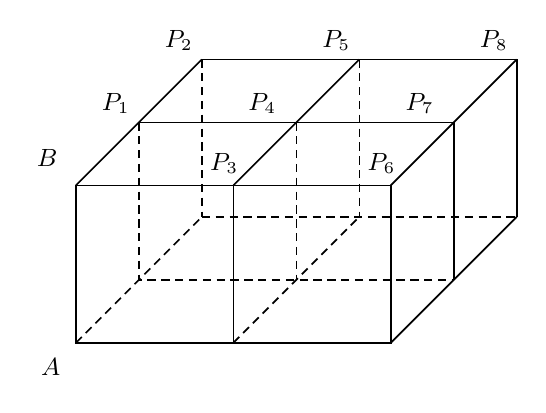
\begin{tikzpicture}[line width=0.6pt, font=\small]
\coordinate (A) at (0,0);
\coordinate (B) at (0,2);
\coordinate (F1) at (2,0);
\coordinate (F2) at (4,0);
\coordinate (P3) at (2,2);
\coordinate (P6) at (4,2);
\coordinate (P1) at (0.8,2.8);
\coordinate (P4) at (2.8,2.8);
\coordinate (P7) at (4.8,2.8);
\coordinate (P2) at (1.6,3.6);
\coordinate (P5) at (3.6,3.6);
\coordinate (P8) at (5.6,3.6);
\coordinate (Ab) at (1.6,1.6);
\coordinate (Fb1) at (3.6,1.6);
\coordinate (Fb2) at (5.6,1.6);
% hidden bottom / back edges (dashed, near bottom)
\draw[densely dashed] (A) -- (Ab);
\draw[densely dashed] (F1) -- (Fb1);
\draw[densely dashed] (Ab) -- (Fb2);
\draw[densely dashed] (P2) -- (Ab);
\draw[densely dashed] (P5) -- (Fb1);
% front face solid
\draw (A) -- (F2) -- (P6) -- (B) -- cycle;
\draw (P3) -- (F1);
% top face solid

\draw (B) -- (P1) -- (P2);
\draw (P3) -- (P4) -- (P5);
\draw (P6) -- (P7) -- (P8);
\draw (P2) -- (P5) -- (P8);
\draw (P1) -- (P4) -- (P7);
% Middle depth row and its three verticals, present in source.
\coordinate (Lmid) at (0.8,0.8);
\coordinate (Mmid) at (2.8,0.8);
\coordinate (Rmid) at (4.8,0.8);
\draw[densely dashed] (P1)--(Lmid)--(Mmid)--(Rmid);
\draw[densely dashed] (P4)--(Mmid);
\draw (P7)--(Rmid);
\draw (F2)--(Fb2);
% right face

\draw (P8) -- (Fb2);
% labels with clearance
\node[below left=2pt] at (A) {$A$};
\node[above left=3pt] at (B) {$B$};
\node[above left=2pt,inner sep=1pt] at (P1) {$P_{1}$};
\node[above left=2pt,inner sep=1pt] at (P2) {$P_{2}$};
\node[above left=2pt,inner sep=1pt,xshift=5pt,yshift=1pt] at (P3) {$P_{3}$};
\node[above left=2pt,inner sep=1pt,xshift=-4pt,yshift=0pt] at (P4) {$P_{4}$};
\node[above left=2pt,inner sep=1pt] at (P5) {$P_{5}$};
\node[above left=2pt,inner sep=1pt,xshift=5pt,yshift=1pt] at (P6) {$P_{6}$};
\node[above left=2pt,inner sep=1pt,xshift=-4pt,yshift=0pt] at (P7) {$P_{7}$};
\node[above left=2pt,inner sep=1pt] at (P8) {$P_{8}$};
\end{tikzpicture}
